\documentclass[12pt]{article}
\usepackage[english]{babel}
\usepackage{natbib}
\usepackage{url}
\usepackage[utf8x]{inputenc}
\usepackage{amsmath}
\usepackage{graphicx}
\graphicspath{{img/}}
\usepackage{parskip}
\usepackage{fancyhdr}
\usepackage{vmargin}
\usepackage{amssymb}
\usepackage{listings}
\usepackage{xcolor}
\usepackage{textcomp}
\usepackage[export]{adjustbox}
\setmarginsrb{3 cm}{2.5 cm}{3 cm}{2.5 cm}{1 cm}{1.5 cm}{1 cm}{1.5 cm}

\title{Lab Report on \\ Basics of MATLAB GUI}			% Title
\author{Rabi Raj Khadka}								% Author
\date{\today}											% Date


\makeatletter
\let\thetitle\@title
\let\theauthor\@author
\let\thedate\@date
\makeatother

\pagestyle{fancy}
\fancyhf{}
\rhead{\theauthor}
\lhead{\thetitle}
\cfoot{\thepage}

\begin{document}

%%%%%%%%%%%%%%%%%%%%%%%%%%%%%%%%%%%%%%%%%%%%%%%%%%%%%%%%%%

\begin{titlepage}
	\centering
%    \vspace*{0.2 cm}
    
\includegraphics[scale = 0.3]{kheclogo.jpg}\\[1.0 cm]	% College Logo
    \textsc{\LARGE Khwopa Engineering College}\\[2.0 cm]	% College Name
	\textsc{\Large Course Code :BEG 475 IP}\\[0.5 cm]				% Course Code
	\textsc{\large Image Processing and Pattern recogntiion}\\[0.5 cm]				% Course Name
	\rule{\linewidth}{0.2 mm} \\[0.4 cm]
	{ \huge \bfseries \thetitle}\\
	\rule{\linewidth}{0.2 mm} \\[3.0 cm]	
	\begin{minipage}{0.4\textwidth}
		\begin{flushleft} \large
			\emph{Author:}\\
			\theauthor
			\end{flushleft}
			\end{minipage}~
			\begin{minipage}{0.4\textwidth}
			\begin{flushright} \large
			\emph{Roll  Number:} \\
			700324									% Your roll Number
		\end{flushright}
	\end{minipage}\\[2 cm]
	
	{\large \thedate}\\[2 cm]
 
	\vfill
	
\end{titlepage}

%%%%%%%%%%%%%%%%%%%%%%%%%%%%%%%%%%%%%%%%%%%%%%%%%%%%%%%%%%

\tableofcontents
\pagebreak

%%%%%%%%%%%%%%%%%%%%%%%%%%%%%%%%%%%%%%%%%%%%%%%%%%%%%%%%%%

\section{Theory:}
\subsection{Gray Level Transformation}
There are three basic gray level transformation.\\
1. Linear\\
2. Logarithmic\\
3. Power – law\\
\begin{figure}[h]
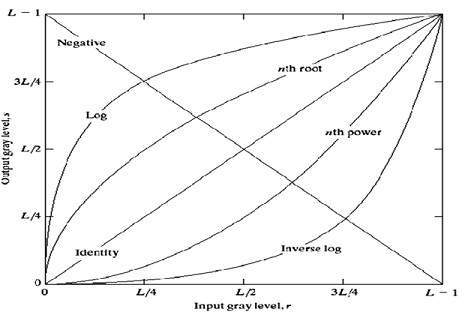
\includegraphics[width=0.5\textwidth, inner ]{graylevelexample.jpg}
\caption{Gray Level Transformatins}
\label{fig:figure1}
\end{figure}

The \textbf{Logarithmic transformations} can be defined by this formula
	$$ s = c  log(r + 1).$$
Where s and r are the pixel values of the output\\ 
and the input image and c is a constant.\\\\
The value 1 is added to each of the pixel value of the input image because if there is a pixel intensity of 0 in the image, then log (0) is equal to infinity. So 1 is added, to make the minimum value at least 1.\\\\
During log transformation, the dark pixels in an image are expanded as compare to the higher pixel values. The higher pixel values are kind of compressed in log transformation, this result in image enhancement and the value of c in the log transform adjust the kind of enhancement we are looking for.\\

The \textbf{Power law transformations} which includes nth power and nth root transformation can be given by the expression:\\
	$$  s=c r^{\Gamma} $$

This symbol $\Gamma$ is called gamma, due to which this transformation is also known as gamma transformation.\\
Variation in the value of $\Gamma$ varies the enhancement of the images. Different display devices/monitors have their own gamma correction, that’s why they display their image at different intensity.\\

This type of transformation is used for enhancing images for different type of display devices. The gamma of different display devices is different. For example Gamma of CRT lies in between of 1.8 to 2.5, that means the image displayed on CRT is dark.\\
Correcting gamma.
\thinspace\thinspace\thinspace \thinspace$s=cr^{\Gamma}\\ \hspace*{4cm}s=cr^{(1/2.5)}$

\subsection{MATLAB GUI}
MATLAB also provides a developer or user to design their application with amazing graphical user interface consisting textbox, axes, push buttons,radio buttons, sliders, inputboxes, popup menus, toggle, table, listbox, panels and manymores.\\

Commands to enter in GUI mode also known as Graphical User Interface Design Environment is \texttt{guide}. 

\pagebreak

\section{Code Description}
\subsection{Program to Demonstrate Gray Level Transformation}
1.Code for Logarithmic and Power Law Transformations\\
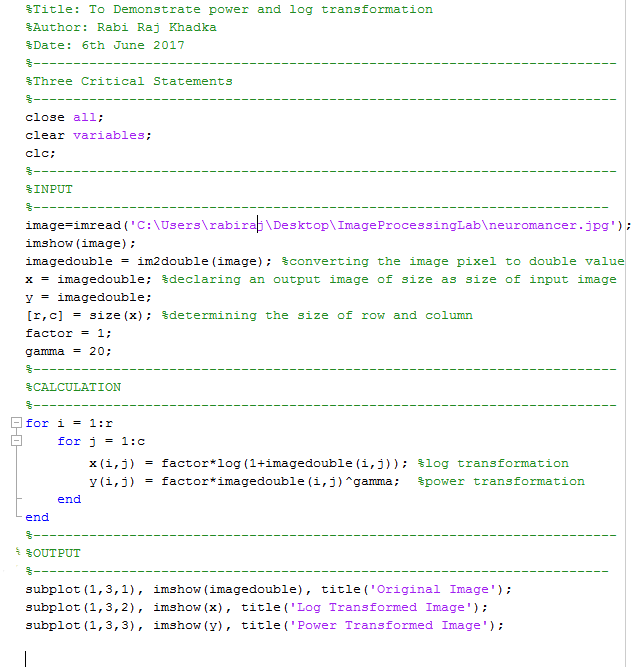
\includegraphics[scale=1.0 ]{3CODEONE.png}

\subsection{Programs to Demonstrate Use of \texttt{GUIDE}}
1.Function to load image using GUI\\

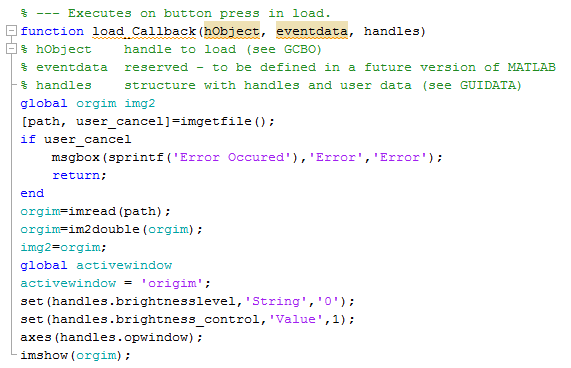
\includegraphics[scale=0.8 ]{3CODETWO.png}

2. Function to convert image into B/W and negative\\


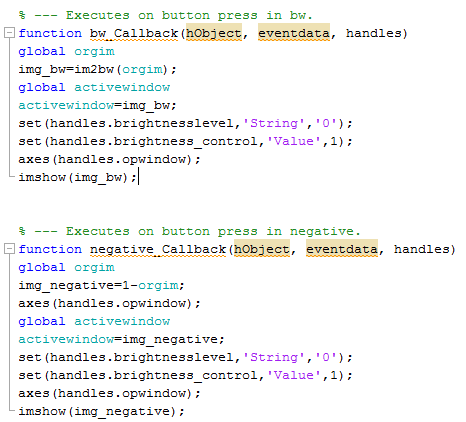
\includegraphics[scale=0.8 ]{3CODETHREE.png}

3. Function to convert image into grayscale, reset original image and control brightness of loaded image \\

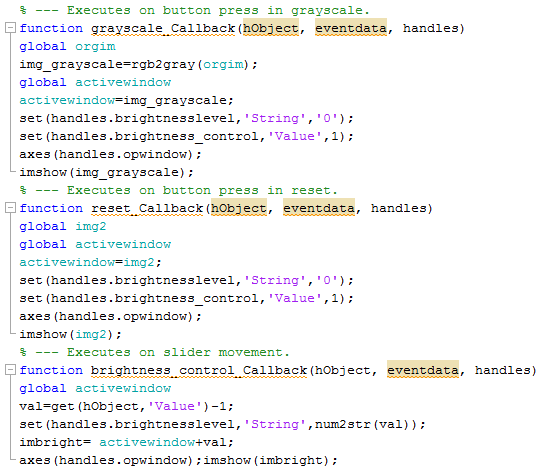
\includegraphics[scale=1.0 ]{3CODEFOUR.png}


\pagebreak

\section{Result and Discussion}
Gray Level Transformation is used for Image enhancement  and we used logarithmic and power law transformations to see how image enhancement is done using Gray level Transformation.\\
The GUI in the MATLAB is easy to use, just by entering "\texttt{guide}" command. There are many functions and interfaces we can use by just dragging and dropping it into design interface. Image is loaded into the UI axes:opwindow and then various operation like converting to black and white, grayscale, negative are done on the copy of original loaded images, for user convenience all active images brightness can be changed through the slider in th right botom of the UI window.\\
\emph{Outputs:}\\

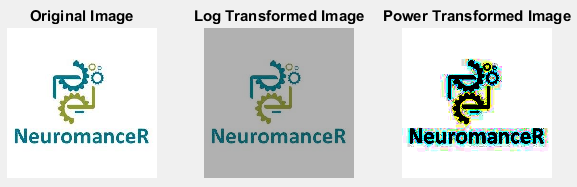
\includegraphics[scale=1.0]{output_labthree_1.png}
{\centering
\texttt{Figure 2:  Gray Level Transformations Example}\par}
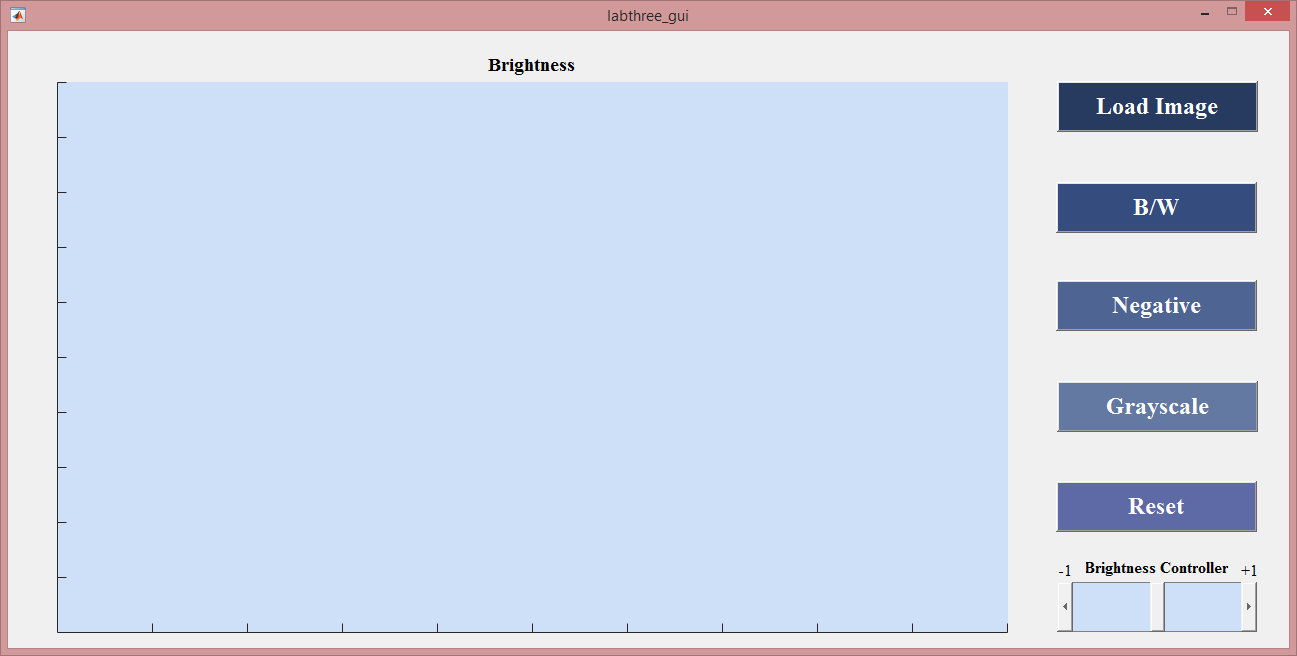
\includegraphics[scale=0.4]{output_labthree_2.png}
{\centering
\texttt{Figure 3: GUI Initial Loaded Window}\par}
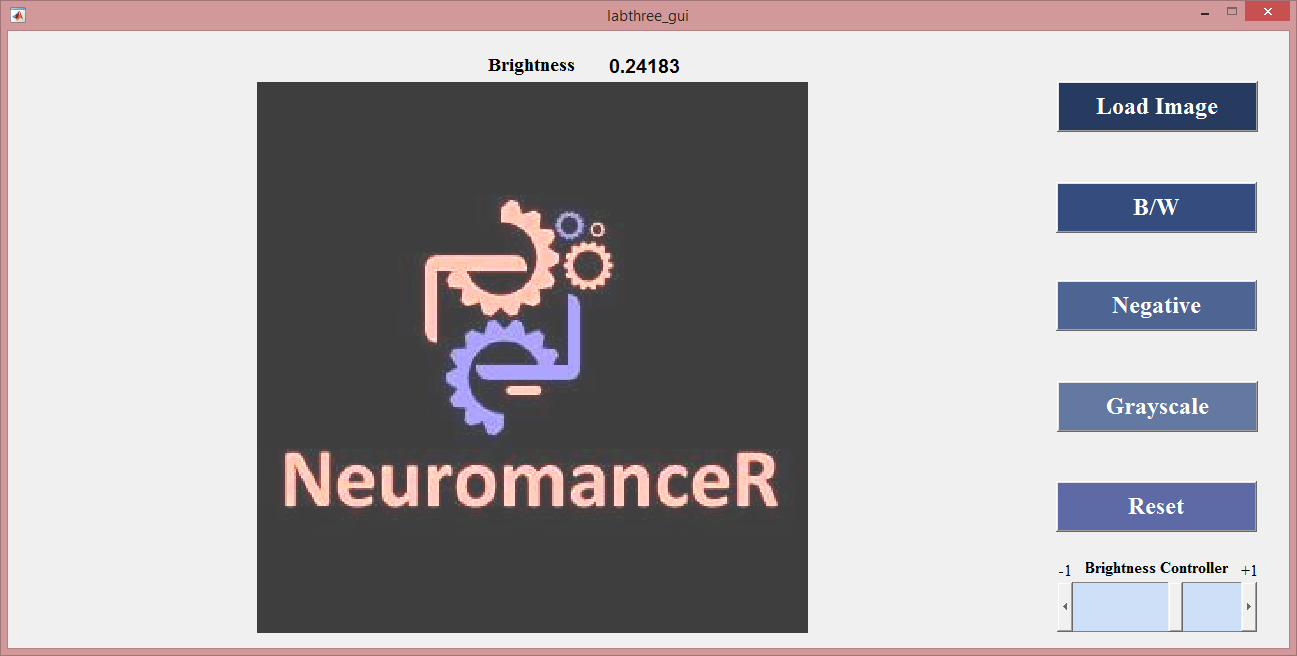
\includegraphics[scale=0.4]{output_labthree_3.png}
{\centering\texttt{Figure 4: GUI example in action}\par}

\pagebreak

\section{Conclusion}
Hence, \\
We are familiarized with the image enhancement techniques and learned about making an GUI based application for windows platform by the use of Graphical User Interface Design Environment of the MATLAB application.

\end{document}